\chapter{Workshop and user testing}

\epigraph{Yeah you wanted a hit \\ but tell me \\ where's the point in it?}{You Wanted a Hit \\ LCD Soundsystem, 2010}

In the past I have taught several classes and crash courses of software of arts, and I used this experience to create a workshop for teaching Tiny Trainable Instruments. Teaching with this thesis project was conceived as a way of user testing and releasing to a wider non-academic audience. In this chapter I explain the workshops's design process, the feedback received from the students, and the challenges faced.

\section{Workshop design}

The Tiny Trainable Instruments workshop primary audience is artists and educators with no previous technical knowledge of programming, \acrshort{ML}, or microcontrollers. It is a hands-on class, where students build their own Tiny Trainable Instruments, create their own databases, and train their own \acrshort{ML} models.

The workshop consists of two sessions of two hours each, taught in two consecutive days for a total of four hours. The first session is focused on installation of the software, connecting the hardware components, and instruments using the color input. The second session is about capturing data and training models, for gesture and speech detection. During both sessions we use different outputs, including serial for text, servo for movement, and buzzer for sound.

This workshop was taught three times, the first two in English for people based in the U.S.A., and the third one in Spanish for people based in Chile. Each workshop had between six and seven students, for a total of twenty students. The three workshops were taught in the span of ten days, and each iteration informed the next one. Between sessions I tweaked the documentation, the class script, and the different code examples to make them easier to understand.

The workshop is designed to be taught virtually or presentially. The students require a laptop computer, internet connection, and a bill of materials for building the Tiny Trainable Instruments. To eliminate cost barriers, I applied and obtained a generous grant of 2,000.00 USD from the \acrlong{CAMIT}. This funding was used to pay for all the materials and shipping for the 20 participants, who signed up, attended for free, and kept the materials to keep on building Tiny Trainable Instruments on their own.

The workshop passed the required approval by the \acrshort{MIT} \acrfull{COUHES}. The workshop didn't ask students to identify themselves, or share any data, and they were always in control of their databases, so this activity complied with the required standards for testing on humans. Additionally, it was taught over videoconferencing software, so all health protocols were respected.

\section{Workshop promotion}

For promoting the workshop I collaborated with designer Renata Gaui \cite{website-renata-gaui}, who designed the bilingual workshop flyers in English and Spanish. I posted these flyers on my Instagram and Twitter accounts, and they were shared by  artists, designers, educators, and activists from different communities in U.S.A. and Chile.

\begin{figure}[ht]
  \centering
  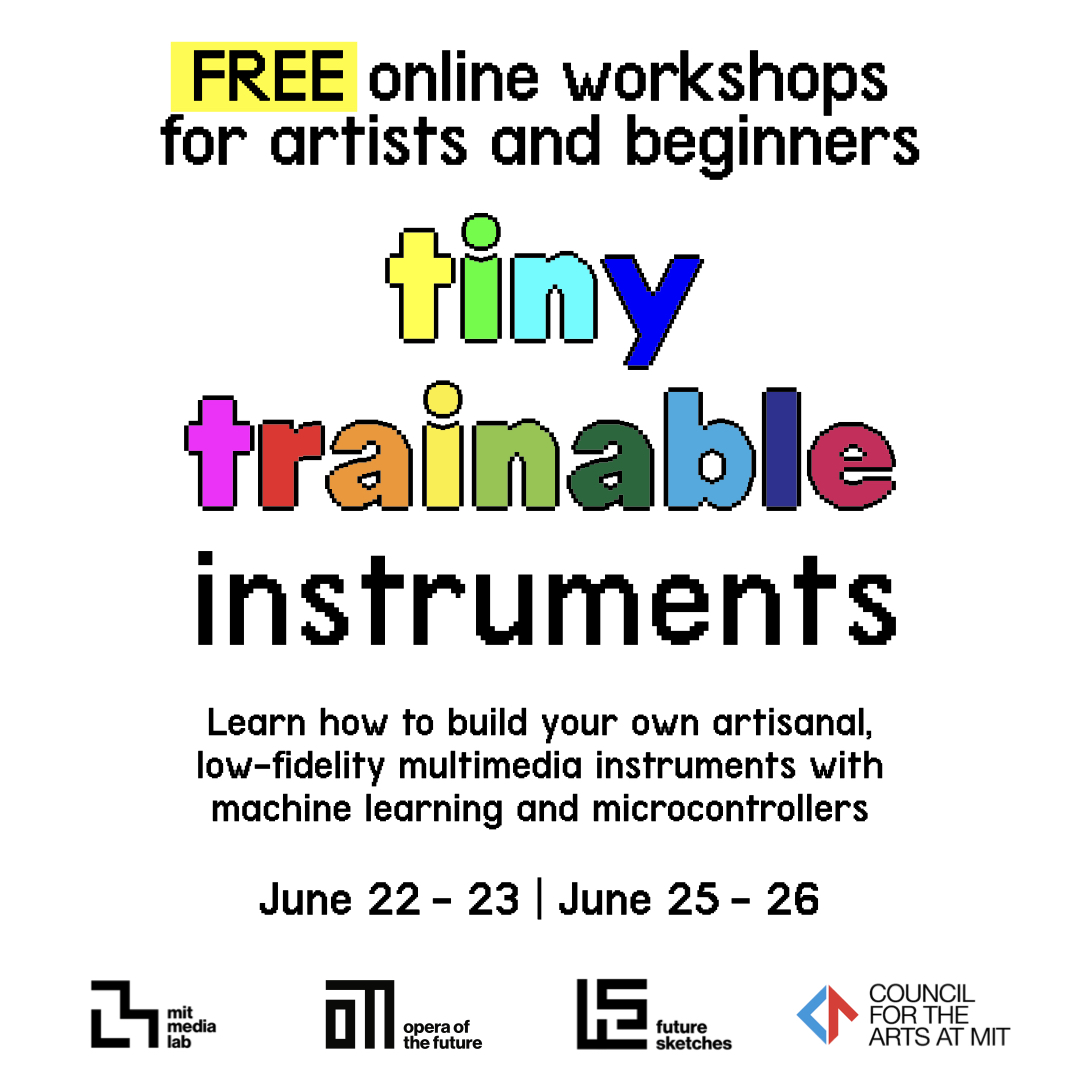
\includegraphics[width=0.75\linewidth,height=0.35\textheight,keepaspectratio]{images/workshop-en-1.jpg}
  \caption{Workshop flyer cover, in English}
  \caption*{Flyer by Renata Gaui}
  \label{fig:workshop-english-flyer-page-1}
\end{figure}

% \begin{figure}[ht]
%   \centering
%   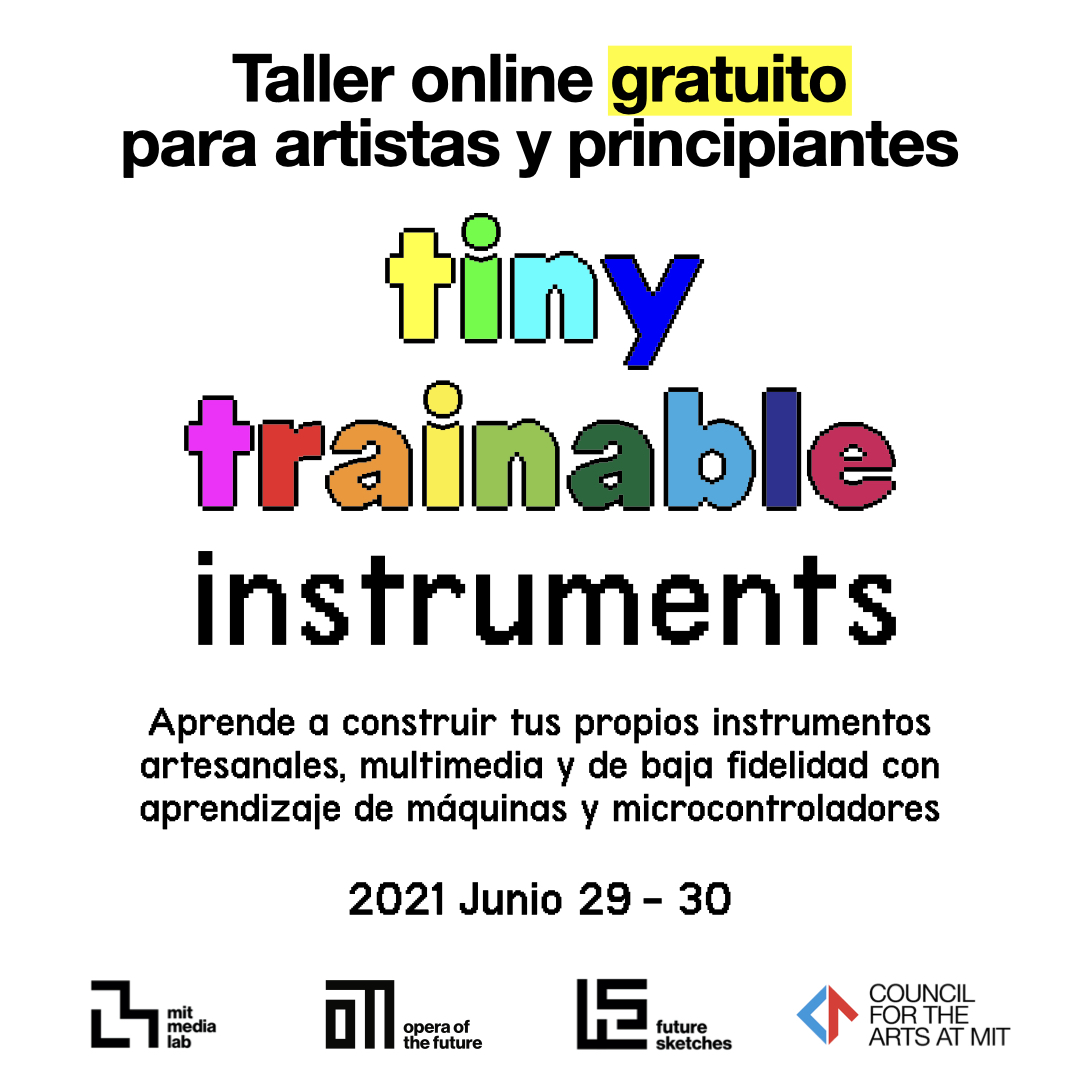
\includegraphics[width=0.75\linewidth,height=0.35\textheight,keepaspectratio]{images/workshop-es-1.jpg}
%   \caption{Workshop flyer cover in Spanish}
%   \caption*{Flyer by Renata Gaui}
%   \label{fig:workshop-spanish-flyer-page-1}
% \end{figure}

The flyers highlighted the multimedia and political orientation of Tiny Trainable Instruments, explaining that in the workshop people would learn how to use \acrshort{ML} with different inputs, including color, gesture and speech, to control different artistic outputs, including text over serial communication, buzzer sounds, and motor movement. The flyer also included a picture of a Tiny Trainable Instruments prototype, made with the Arduino microcontroller on a breadboard, jumper wires, a servo motor, and masking tape, to foster an artisanal and welcoming environment for beginners.

% \begin{figure}[ht]
%   \centering
%   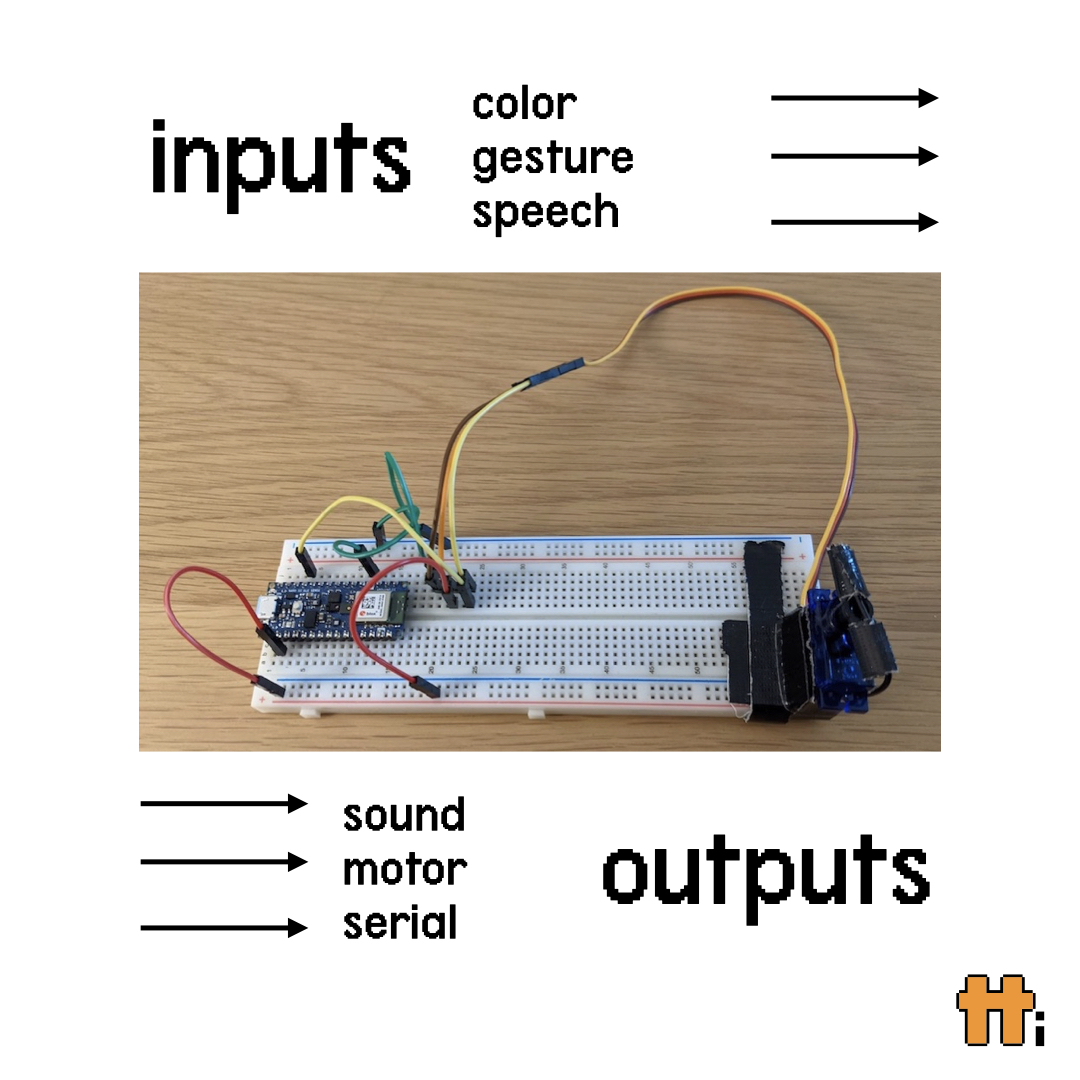
\includegraphics[width=0.75\linewidth,height=0.35\textheight,keepaspectratio]{images/workshop-en-2.jpg}
%   \caption{Workshop flyer multimedia output in English}
%   \caption*{Flyer by Renata Gaui}
%   \label{fig:workshop-english-flyer-page-2}
% \end{figure}

\begin{figure}[ht]
  \centering
  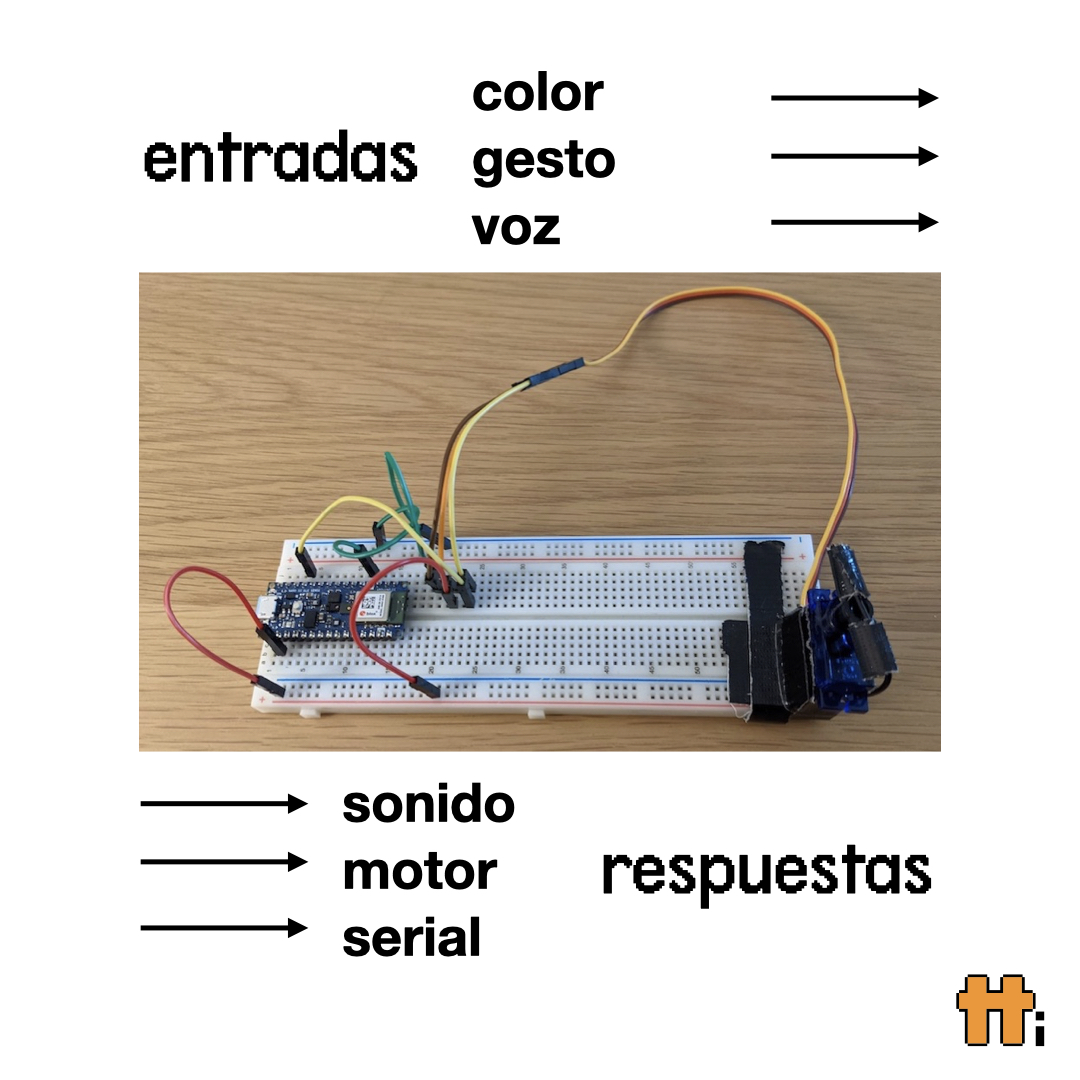
\includegraphics[width=0.75\linewidth,height=0.35\textheight,keepaspectratio]{images/workshop-es-2.jpg}
  \caption{Workshop flyer multimedia inputs and outputs, in Spanish}
  \caption*{Flyer by Renata Gaui}
  \label{fig:workshop-spanish-flyer-page-2}
\end{figure}

More than ninety people signed up for the twenty available spots. I consider this open call to be succesful, since it reached people who I didn't know at all who were entushiastic about this project. I picked the twenty students, so that I could have a diverse crowd, including artists, designers, musicians, programmers, educators, and activists. I included some acquaintances and former students, with the hope to get deeper feedback from them during and after the workshop. It also helped me to have more confidence while teaching on this new virtual format, and after a one year hiatus of organizing workshops.

The three workshops were taught respectively on June 22-23, June 25-26, and June 29-30 2021.

\section{Workshop logistics}

Before each workshop, the participants are sent a basic kit for building Tiny Trainable Instruments, including these six elements: Arduino microcontroller, breadboard, jumper wires, USB cable, buzzer, servo motor.

The first four materials are needed for any Tiny Trainable Instruments, and the last two were picked for outputting sound and movement, to appeal to a wide audience of artists. They were also selected over others, because of their simple wiring and cheap cost, compared to the other outputs supported by the software library.

The Arduino microcontroller can be acquired from the Arduino online store, or from other electronics distributors. The rest of the materials are available on Adafruit, picked because of its focus on being an electronics store for artists and beginners.

For the thirteen students in the U.S.A. I acquired the materials from sellers Arduino and Adafruit, and then shipped them to their addressses their kits via \acrfull{USPS}.

\begin{figure}[ht]
  \centering
  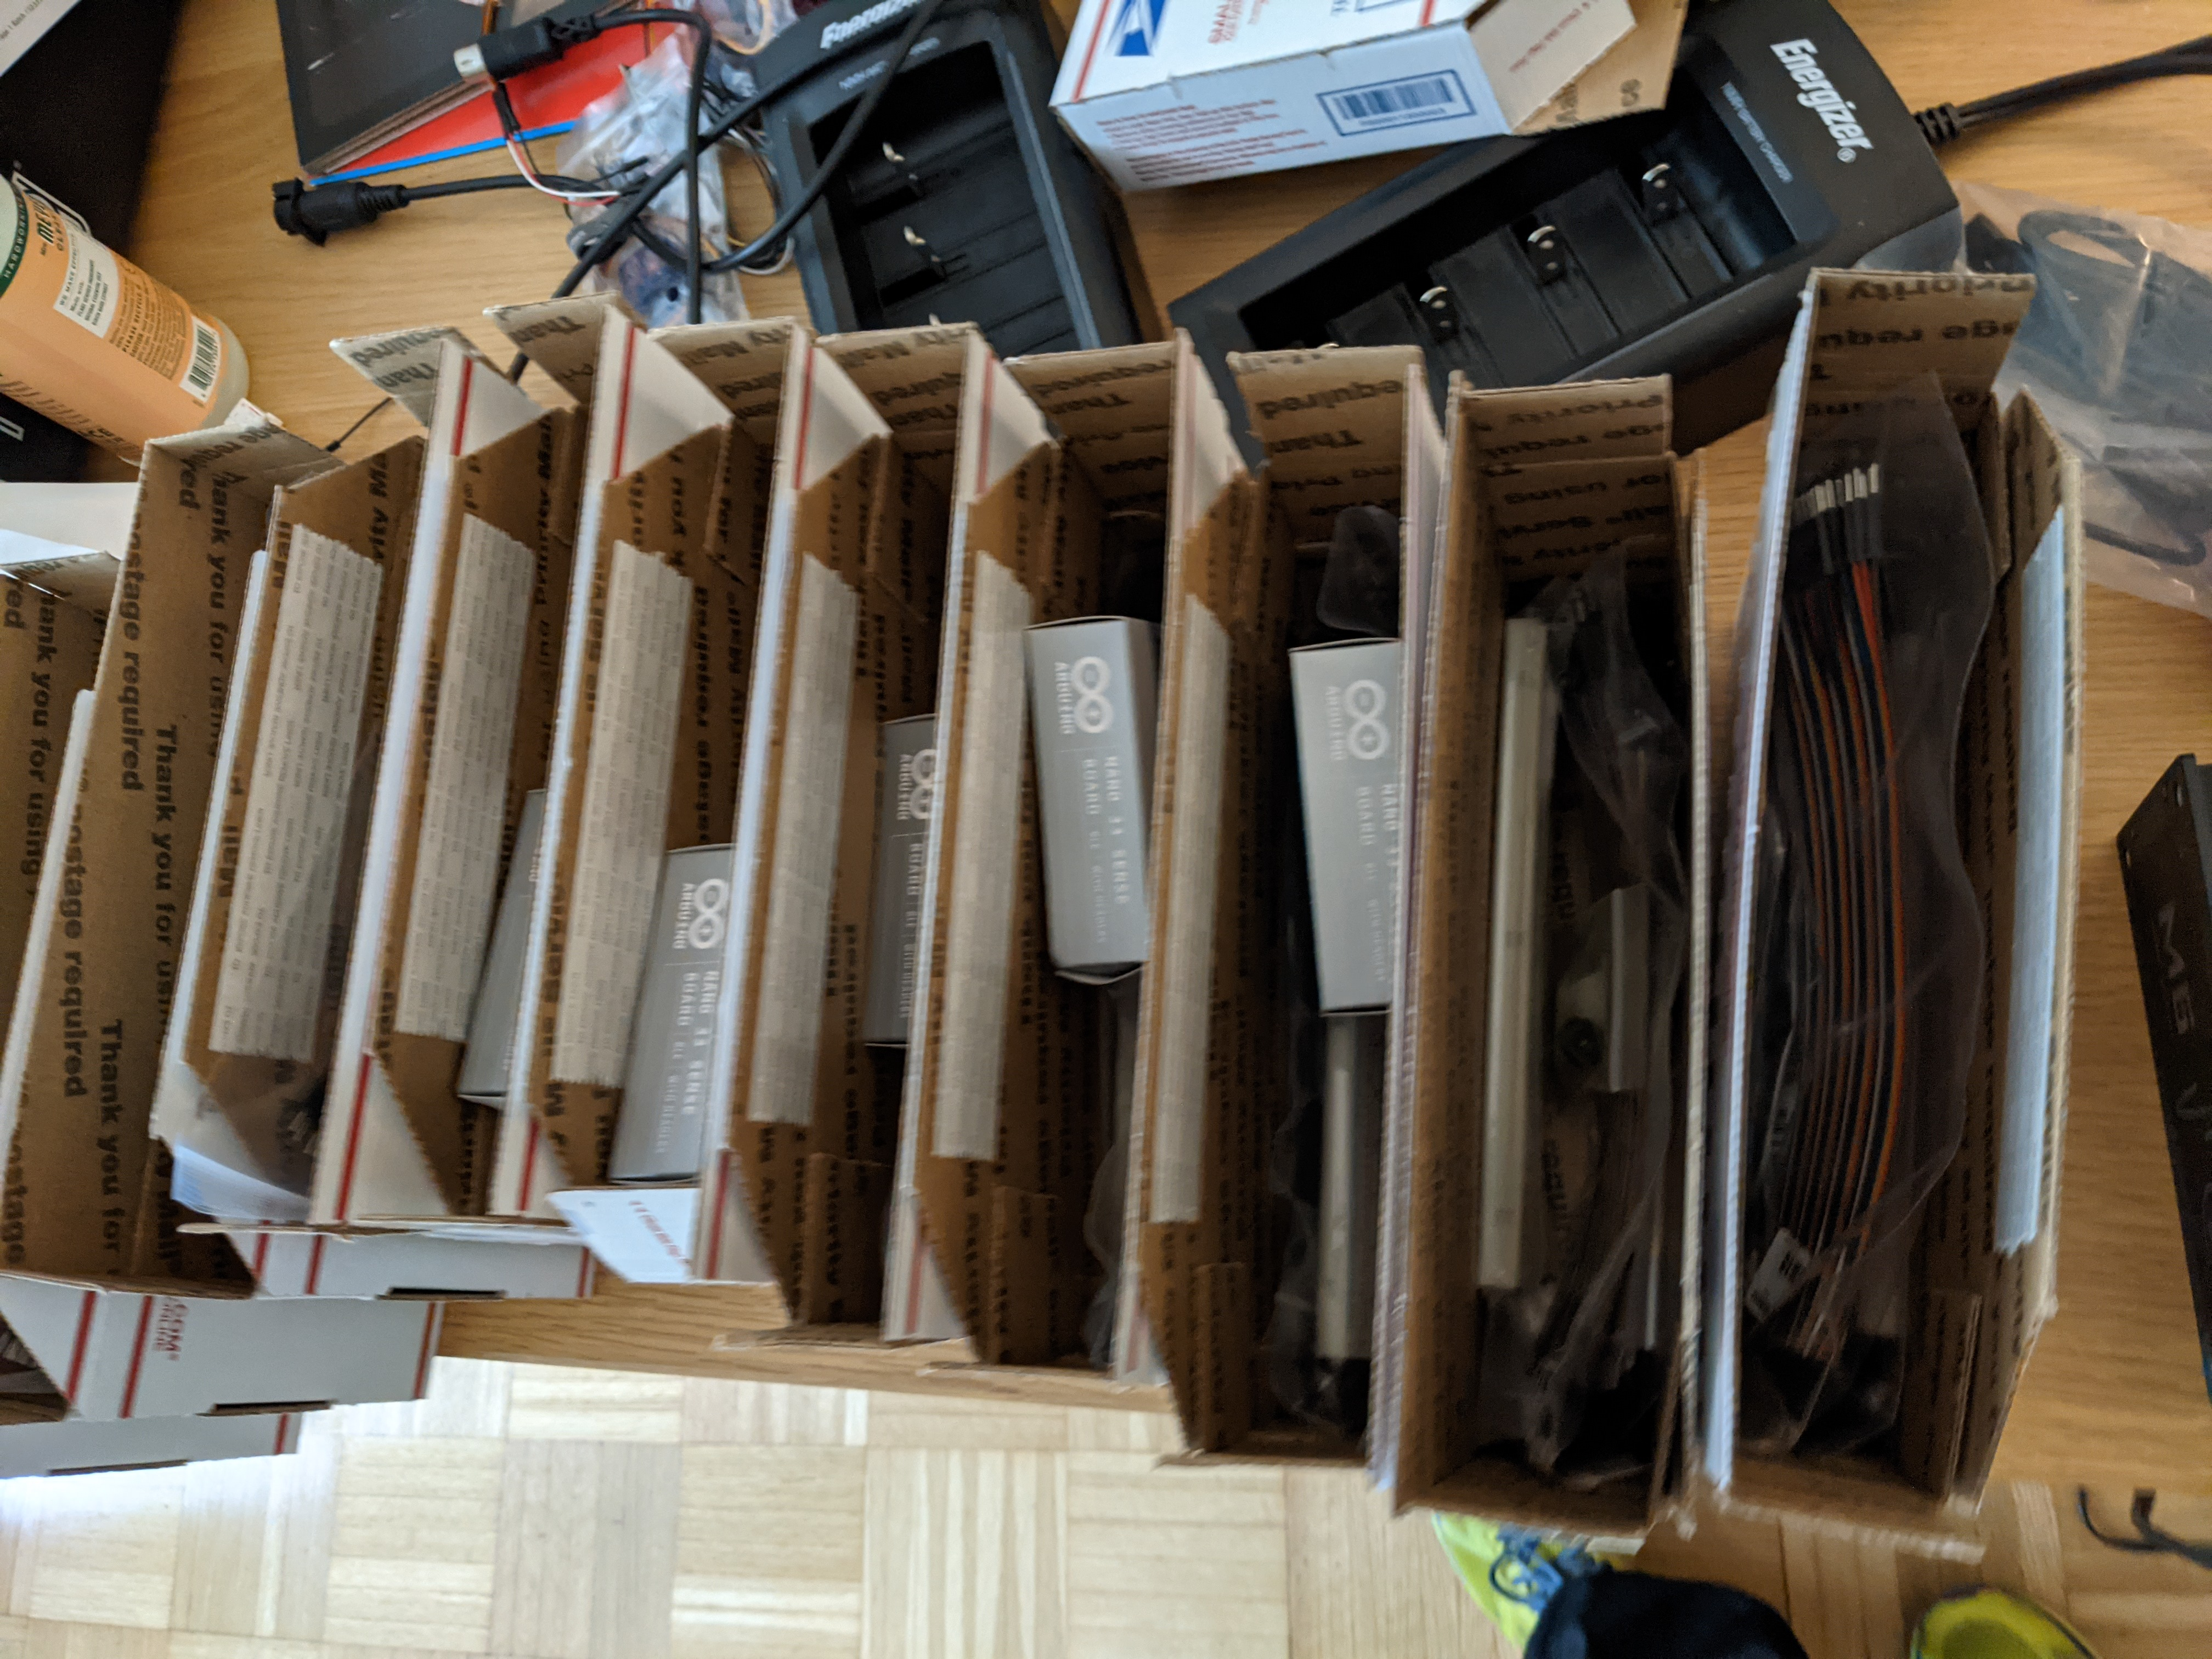
\includegraphics[width=0.75\linewidth,height=0.25\textheight,keepaspectratio]{images/workshop-packages.jpg}
  \caption{Workshop packages for the students in U.S.A.}
  \caption*{Picture by myself}
  \label{fig:workshop-packages-usa}
\end{figure}

For the seven students in Chile, I acquired the materials from the same vendor, and shipped them to my mother's home in Chile. She also sorted them in kits and then distributed them to the participants, via pickup or mail.

\begin{figure}[ht]
  \centering
  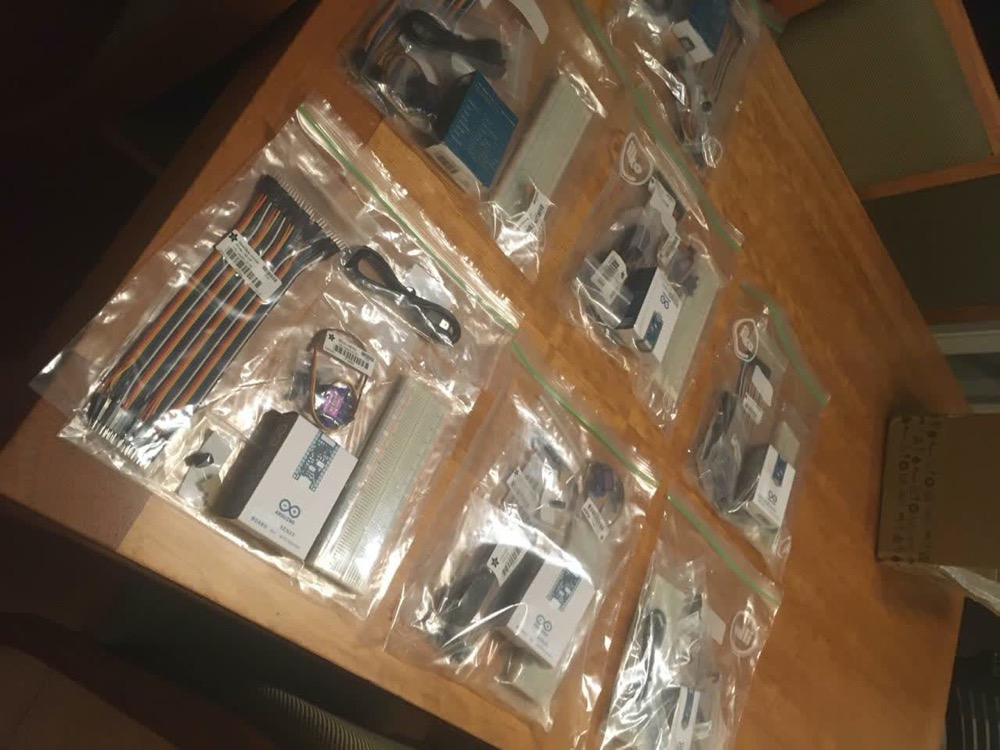
\includegraphics[width=0.75\linewidth,height=0.25\textheight,keepaspectratio]{images/workshop-packages-chile.jpg}
  \caption{Workshop packages for the students in Chile}
  \caption*{Picture by Bernardita Moraga}
  \label{fig:workshop-packages-chile}
\end{figure}

In parallel to the shipping to the materials, the participants were sent instructions via email, with links to the project's documentation, in particular to install the Arduino \acrshort{IDE}.

In the first session we will first help people with installation of the software, and then move on to start wiring the materials on the electronic breadboard material. We will concentrate on the simpler examples with color input. We will also collect data of gesture and speech to create custom databases and use them to train other slow machine learning models that will keep on running on the student's workshops after the workshop is over.

In the second session we will use the result of the trained models to create more advanced instruments that react to gesture and speech. We will also show the participants the other 


what did participants create

what challenges did they face

what did they find most interesting

\section{Workshop feedback}

After the completion of the workshops I sent the students a Google form to ask for anonymous feedback. Here are some of the results.

Students called the workshop interesting, challenging, fun, innovative, inspiring, didactical, exciting, fun, new, fast-paced, and experimental.


what changes did they suggest, etc.

Did the workshops provide you with new ideas on how to modify the TinyTrainable library in the future? Or new ideas on how to introduce the library to beginners?



The workshop instructions are documented on the docs/ folder of the repository available at \url{https://github.com/montoyamoraga/tiny-trainable-instruments}

Each workshop consists of 2 sessions of 2 hours each, spread over 2 consecutive days.


\section{Multimedia documentation}

TODO: upload a collection of examples made by people who came to the workshops, featuring the software library and what they learned.
